% Document geometry and pre-requisites
\documentclass[12pt]{article}
\usepackage[a4paper, margin=2cm]{geometry}
\usepackage{tikz}
\usetikzlibrary{matrix, positioning}

\newcommand{\n}{\textbf{N}}
\renewcommand{\v}{\textbf{V}}
\renewcommand{\d}{\textbf{D}}

\begin{document}
\section{Default}
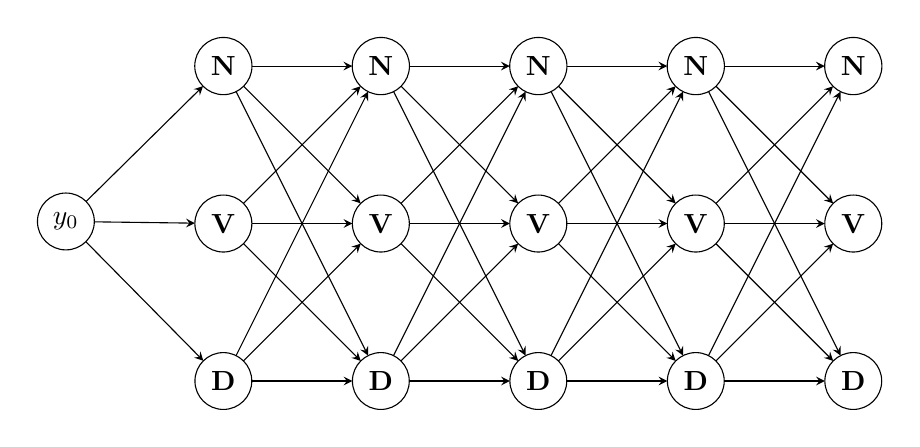
\begin{tikzpicture}
  \matrix (network)
    [matrix of nodes,%
     nodes in empty cells,
     nodes={outer sep=0pt,circle,draw},
     column sep={2cm,between origins},
     row sep={2cm,between origins}]
  {
    |[draw=none]| & \n & \n & \n & \n & \n \\
    |[yshift=3pt]| $y_0$ & \v & \v & \v & \v & \v \\
    |[draw=none]| & \d & \d & \d & \d & \d \\
  };
  \foreach \y in {1,2,3}{
    \draw [-stealth] (network-2-1) -- (network-\y-2);
  };

  \foreach \x [evaluate=\x as \nextx using int(\x+1)] in {2,...,5}{
    \foreach \y in {1,2,3}{
    \foreach \i in {1,2,3}{
    \draw [-stealth] (network-\y-\x) -- (network-\i-\nextx);
    };
    };
    };
  
\end{tikzpicture}
\section{Forward-Variable}
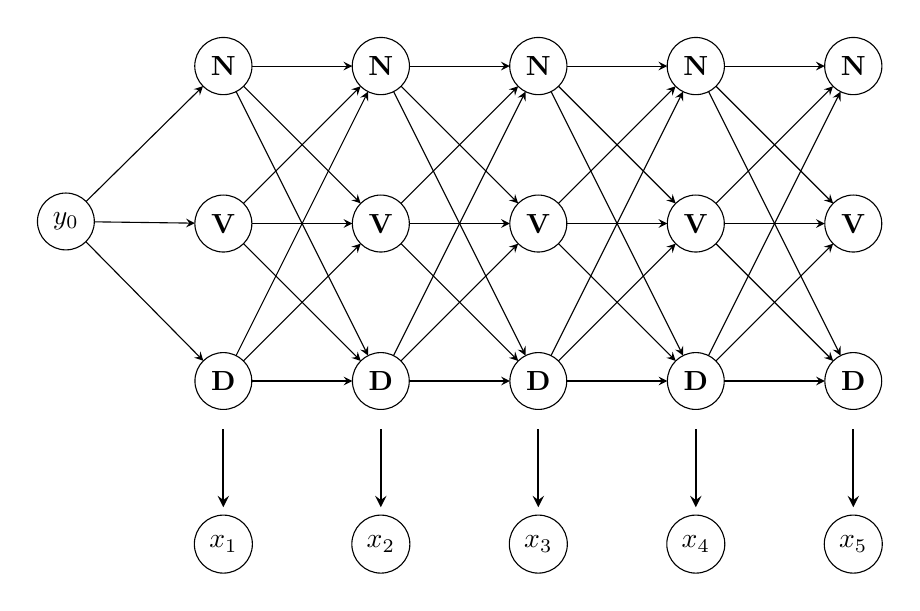
\begin{tikzpicture}
  \matrix (network)
    [matrix of nodes,%
     nodes in empty cells,
     nodes={outer sep=0pt,circle,draw},
     column sep={2cm,between origins},
     row sep={2cm,between origins}]
  {
    |[draw=none]| & \n & \n & \n & \n & \n \\
    |[yshift=3pt]| $y_0$ & \v & \v & \v & \v & \v \\
    |[draw=none]| & \d & \d & \d & \d & \d \\
    |[draw=none]| & $x_1$ & $x_2$ & $x_3$ & $x_4$ & $x_5$ \\
  };
  \foreach \y in {1,2,3}{
    \draw [-stealth] (network-2-1) -- (network-\y-2);
  };

  \foreach \x [evaluate=\x as \nextx using int(\x+1)] in {2,...,5}{
    \foreach \y in {1,2,3}{
    \foreach \i in {1,2,3}{
    \draw [-stealth] (network-\y-\x) -- (network-\i-\nextx);
    };
    };
    };

    \foreach \x in {2,...,6}{
        \draw [-stealth, shorten <= 0.25cm, shorten >= 0.1cm, thick] (network-3-\x) -- (network-4-\x);
    };
  
\end{tikzpicture}

\section{Final-Trellis}
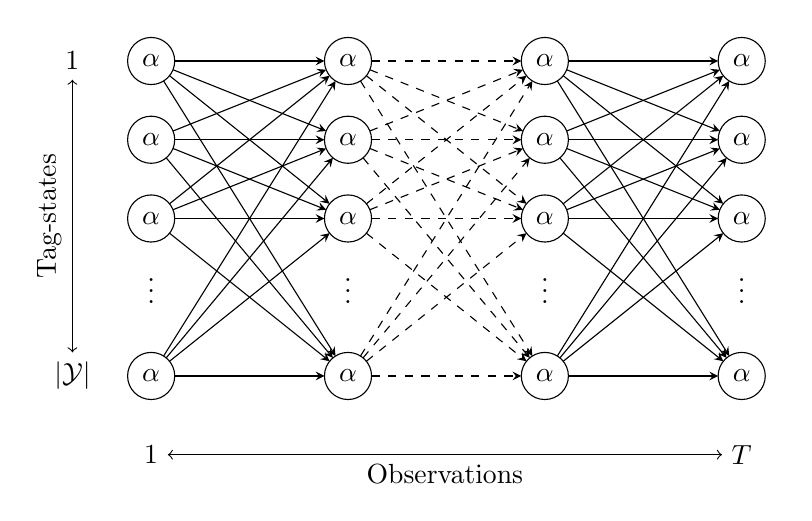
\begin{tikzpicture}
  \matrix (network)
    [matrix of nodes,%
     nodes in empty cells,
     nodes={outer sep=0pt,circle,draw},
     column sep={2.5cm,between origins},
     row sep={1cm,between origins}]
  {
    $\alpha$ & $\alpha$ & $\alpha$ & $\alpha$ \\
    $\alpha$ & $\alpha$ & $\alpha$ & $\alpha$ \\
    $\alpha$ & $\alpha$ & $\alpha$ & $\alpha$ \\
    |[draw=none]| $\vdots$ & |[draw=none]| $\vdots$ & |[draw=none]| $\vdots$ & |[draw=none]| $\vdots$ \\
    $\alpha$ & $\alpha$ & $\alpha$ & $\alpha$ \\
  };
  \foreach \x [evaluate=\x as \nextx using int(\x+1)] in {1,3}{
    \foreach \y in {1,2,3,5}{
    \foreach \i in {1,2,3,5}{
    \draw [-stealth] (network-\y-\x) -- (network-\i-\nextx);
    };
    };
    };

  \foreach \y in {1,2,3,5}{
    \foreach \i in {1,2,3,5}{
    \draw [-stealth, dashed] (network-\y-2) -- (network-\i-3);
    };
    };

    \node [below of=network-5-1] (obs1) {$1$};
    \node [below of=network-5-4] (obsT) {$T$};
    \draw[<->] (obs1) -- (obsT) node [midway, below] {Observations};

  \node [left of=network-1-1] (state1) {$1$};
  \node [left of=network-5-1] (stateY) {$|\mathcal{Y}|$};
  \draw[<->] (state1) -- (stateY) node [midway, left, rotate=90, anchor=base, yshift=6pt] {Tag-states};
\end{tikzpicture}
\end{document}